\section{Framework}
\KZ{Preamble goes here.. Give an overview of this section first..}

\subsection{Representing the code}

We propose a new kind of Recursive Neural Network called Code-RNN to mine the information of source codes' parse tree. Our Code-RNN is the arbitrary tree form while other Recursive Neural Network used in NLP is binary tree form. Fig. \ref{fig:code_rnn} shows an example of Code-RNN.

Exactly, the Code-RNN is the parse tree of source code but we make it the neural network now. We use JavaParser\footnote{The source code of JavaParser can be downloaded from web https://github.com/javaparser/javaparser.} to generate parse tree. We add the root node in the parse tree at first, then we add statements as the children of root node. In Fig. \ref{fig:code_rnn}, we can see the code snippet has two if statement, so the root node has two same children. We only show the detail of second if statement and the ``......' represents all nodes of the first if statement. For the if statement, it has the three children statements, ``Condition'',``ThenStmt'' and ``ElseStmt''. In this example, it don't have the children ``ElseStmt'' so we don't put it in the parse tree. Then we can construct our parse tree recursively. And we add a new inter-node ``CombineName'' to show that the children of it are combined together in the source code. We add this inter-node to extract more identifier semantics and make the size of vocabulary smaller. In this example, we split ``allFound'' into ``all'' and ``found'' according to the capital character. About identifier semantics, we will discuss more details in Section \ref{sec:identifier}.

In Code-RNN, every node has its own unique vector representation $V_{c}$, and there are sharing parameters $W$ and bias $b$, these three kinds of parameter are tuned during training process.

According to different way of calculating vector representation, we propose \textbf{Sum Model} and \textbf{Average Model}. The equations of calculating vector representation are as follows.

\begin{figure*}[th]
\begin{minipage}{0.15\linewidth}
  \begin{lstlisting}

  if (!found){
    allFound = false;
  }
  if (allFound){
    return true;
  }
\end{lstlisting}
 \centerline{source code}
\end{minipage}
\hfill
\begin{minipage}{0.9\linewidth}
  \centering
	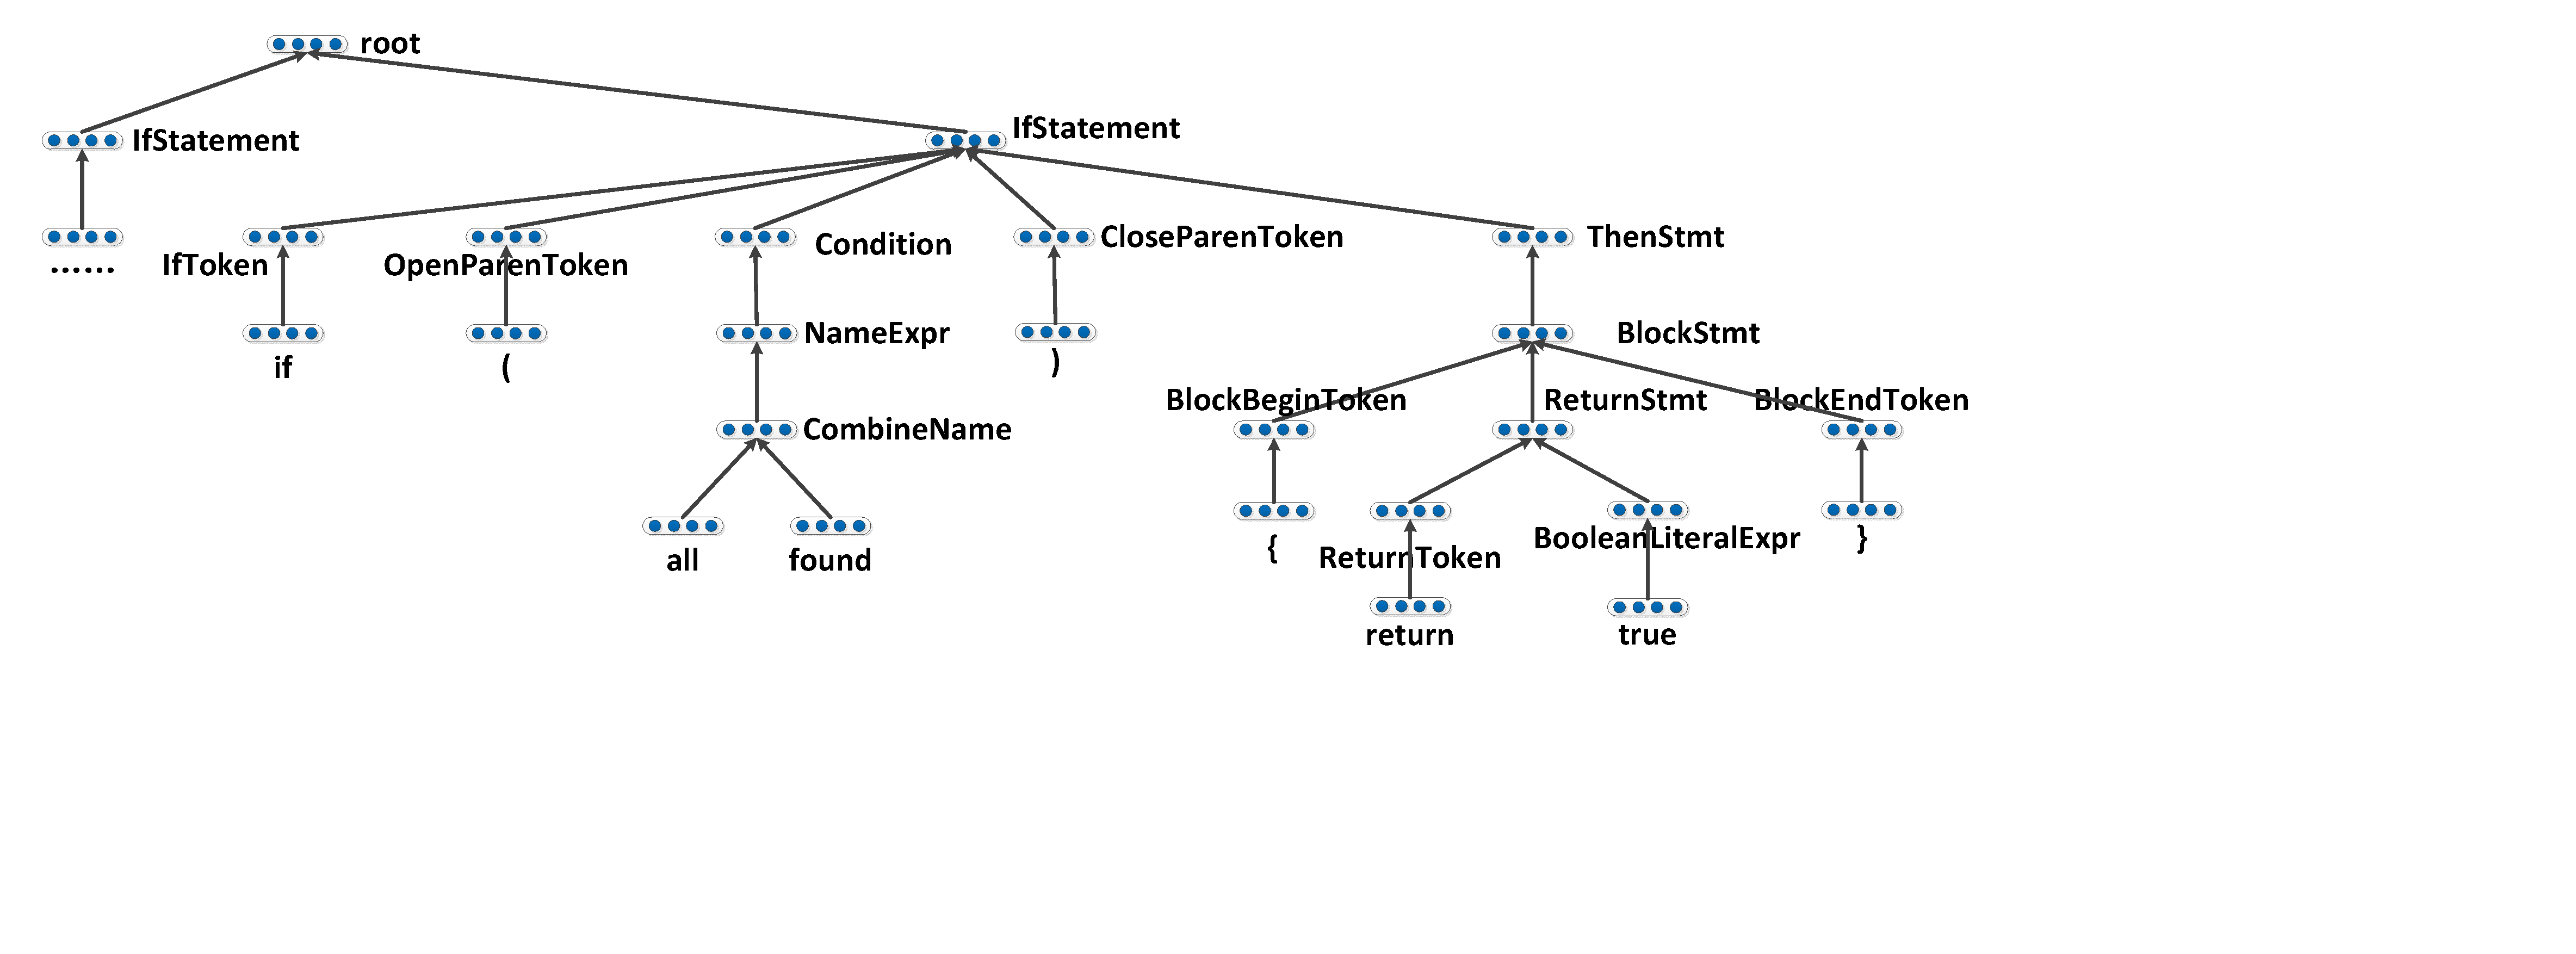
\includegraphics[width=0.9\linewidth]{img/tree_rnn.pdf}
 \centerline{Code-RNN}
\end{minipage}

\caption{Code-RNN Example}\label{fig:code_rnn}
\end{figure*}

\subsubsection{Sum Model}

\begin{equation}\label{eq:code_rnn_sum}
V = V_{node} + f(W \times \sum_{c \in C}{ V_{c}} + b)
\end{equation}

\subsubsection{Average Model}

\begin{equation}\label{eq:code_rnn_average}
V = V_{node} + f(W \times \frac{1}{n}\sum_{c \in C}{V_{c}} + b)
\end{equation}

$V$ is the new representation vector, $V_{node}$ is the unique vector for every node type, $n$ is the number of children nodes, $c$ is the index of children node type, and $C$ is the index set. $W$ is the weight matrix and $b$ is the bias and all nodes are the same. $f$ is \textbf{RELU} activation function.

We use these equations to through the whole Code-RNN at every inter-node. Finally get the vector of root node and think it as the vector of the method.

\subsubsection{Identifier Semantics}\label{sec:identifier}
%\KZ{\textcolor{red}{This section needs to be expanded significantly. I still don't understand
%Table \ref{table:abbr}. If you use rules, you should explicitly say what those
%rules are to recover the original words from the abbreviations. If you use
%some algorithm, better include the listing of the pseudo-code.}}

\begin{table}[th]
\centering
\scriptsize{
\caption{\label{table:splitID} Example of Split Identifiers}
\begin{tabular}{|c|c|}
\hline
Identifier & Words \\
\hline
contextInitialize & context, initialize\\
\hline
apiSettings & api, settings\\
\hline
buildDataDictionary & build, data, dictionary\\
\hline
add\_result & add, result\\
\hline
\end{tabular}
}
\end{table}

\begin{table}[ht]
\centering
\scriptsize{
\caption{Example of Abbreviation}
\label{table:abbr}
\begin{tabular}{|c|c|c|}
\hline
Abbreviation & Origin & Context\\
\hline
val & value & key.value()\\
\hline
cm & confusion, matrix & new ConfusionMatrix()\\
\hline
conf & configuration & context.getConfiguration()\\
\hline
rnd & random & RandomUtils.getRandom()\\
\hline
\end{tabular}
}
\end{table}

In this work, we adopt two ways that extract the semantics from the identifiers.
One is to split all the long forms to multiple words and
the other one is to recover the full words from abbreviations.

Table \ref{table:splitID} shows some example identifiers and the results
of splitting. Many identifiers in the source code are combination of English words,
with the first letter of the word in upper case, or joined together using
underscores. We thus define simple rules to extract the original
English words accordingly.
To show these words are one word in the source code, we add a new inter-node in Code-RNN, ``CombineName'', Fig. \ref{fig:code_rnn} also has this node.

For example, we can split the expression ``DoubleMatrix(confusionMatrix)''
into two lists. The first list contains ``double'' and ``matrix'',
and the second contains ``confusion'' and ``matrix''.

Table \ref{table:abbr} shows some abbreviations and
their original version. We can infer the complete words by
looking for longer forms in the context of the identifier in the code.
Specifically, we compare the identifier with the word list generated from
the context of the identifier to see whether the identifier's name
is a substring of some word from the list, or is the combination of
the initial of the words in the list.
If the list contains only one word, we just check if the identifier
is part of that word. If so, we conclude that the identifier is the
abbreviation of that word with higher probability.
In the second situation, we can collect all the initials of the words
in the list together to see whether the identifier is part of
this collection. Suppose the code fragment is

\begin{lstlisting}
Matrix dm = new DoubleMatrix(confusionMatrix);
\end{lstlisting}
%After this process we can get most of the full names of the parameters.
We search for the original words of ``dm'' as follows.
At beginning, we see ``dm'' is not the substring of any word in any list
we establish. Then we collect the initials of the words in one list and
get three collections ``m'' ``dm'' and ``cm''.
Consequently, ``dm'' is an abbreviation of ``DoubleMatrix''.

\subsubsection{Training}
When we train the Code-RNN, we begin from all leaf nodes. We use the node ``CombineName'' in Fig. \ref{fig:code_rnn} as an example. Now we totally have three vectors $V_{all}$, $V_{found}$ and $V_{CombineName}$ with respect to node ``all'', ``found'' and ``CombineName''. For node ``CombineName'', it has two children ``all'' and ``found'', so the vector representation $V_{train\_CombineName}$ of node ``CombienName'' during training will be calculated as $V_{CombineName} + f(W \times (V_{all} + V_{found}) + b)$ in Sum Model or $V_{CombineName} + f(W \times 0.5 \times (V_{all} + V_{found}) + b)$ in Average Model. Then we can get the vector representation $V_{train\_NameExpr}$ of the parent of node ``CombineName'', ''NameExpr'', during training. Recursively, we can get the vector of node ``root'' as $V_{train\_root}$, and we regard $V_{train\_root}$ as the vector representation of the whole method.

For classification problem, we apply $softmax$ function to $V_{train\_root}$ to train. During back-propagation process, we through the whole network from root node to all leaf nodes recursively and tune all parameters in Equation \ref{eq:code_rnn_sum} and Equation \ref{eq:code_rnn_average} except $n$ to approach to the best situation.

\subsubsection{Test}

No matter what problem we want to solve, we can use our Code-RNN model to get a meaningful vector representation of methods or parse trees, just repeat the forward-propagation of training time and get the vector representation of root node $V_{train\_root}$. Then we can use this vector to do following works such as classification problem and comment generation. More details will be discussed later.

To see the contribution of structure information and natural language, 
we propose two other models as the baselines. \KZ{I think these two
baselines can go into eval section.}

\subsection{Inter-node Code-RNN}

\KZ{This section is too short and not sure what you are trying to say.}
This model delete all leaf nodes of original Code-RNN that means the text in the source code are all deleted from parse tree and the neural network only contains structure information of source code now. And this model's structure and equations are same as \textbf{Code-RNN}. Forward-propagation and back-propagation are like Code-RNN too.

\subsection{Language Embedding}

Language embedding model only use text information of source code so no parse tree in this model. We firstly extract all words except all special symbols (``\$'', ``('', ``+'', $\cdots$) in the source codes and construct word bags for every methods. We also split all the long forms to multiple words as mentioned before. Then every single word will have an unique vector representation and this vector will be tuned during training. This model also has two sub-models \textbf{Sum Model} and \textbf{Average Model}.

\subsubsection{Sum Model}
\begin{equation}
V = \sum_{w \in W}{V_{w}}
\end{equation}

\subsubsection{Average Model}

\begin{equation}
V = \frac{1}{n}\sum_{w \in W}{V_{w}}
\end{equation}
where $V$ is the vector representation of one method, $W$ is the word bag of this method and $w$ is one word in word bag, $V_{w}$ is the vector representation of word $w$, and $n$ is the number of words in word bag $W$.

%\begin{equation}
%V = \left[
%\begin{matrix}
%V_{tree}\\
%V_{word}
%\end{matrix}
%\right] \times W
%\end{equation}


\subsection{Comment Generation}
A. Karpathy and L. Fei-Fei~\cite{karpathy2015deep} proposed a meaningful method to generate image descriptions. In their model, they connect CNN and RNN(Recurrent Neural Network) end-to-end to generate description. This is different from other language model based on Recurrent Neural Network \cite{elman1990finding}\cite{sutskever2011generating}\cite{mikolov2010recurrent}, they generate sentences by defining a probability distribution of the next word in a sequence given the current word and context from previous time steps. We also use this model but replace CNN to our model Code-RNN, and feed Code-RNN vector in every step of RNN(Recurrent Neural Network). Fig. \ref{fig:comment_generate} shows our comment generation process.

We use pre-trained model Code-RNN to get the representation vector of methods $V_{Code\_RNN}$. This vector $V_{Code\_RNN}$ won't be tuned during training of comment generation model. Then we feed method vector into the RNN(Recurrent Neural Network) model at every step. For example in Fig.~\ref{fig:comment_generate}, we input the START token as the beginning input of model and feed the method vector into hidden layer. After calculating the output of this step, we do the back-propagation. Then we begin the second step. We input the word ``gets'' and feed the method vector $V_{Code\_RNN}$ into hidden layer again, this is different from A. Karpathy and L. Fei-Fei~\cite{karpathy2015deep}, and receive the $h_{t-1}$ from the first step. Then we repeat the procession mentioned above to tune parameters. The equations of comment generation model are listed below.

\begin{figure}[!htb]
\centering
	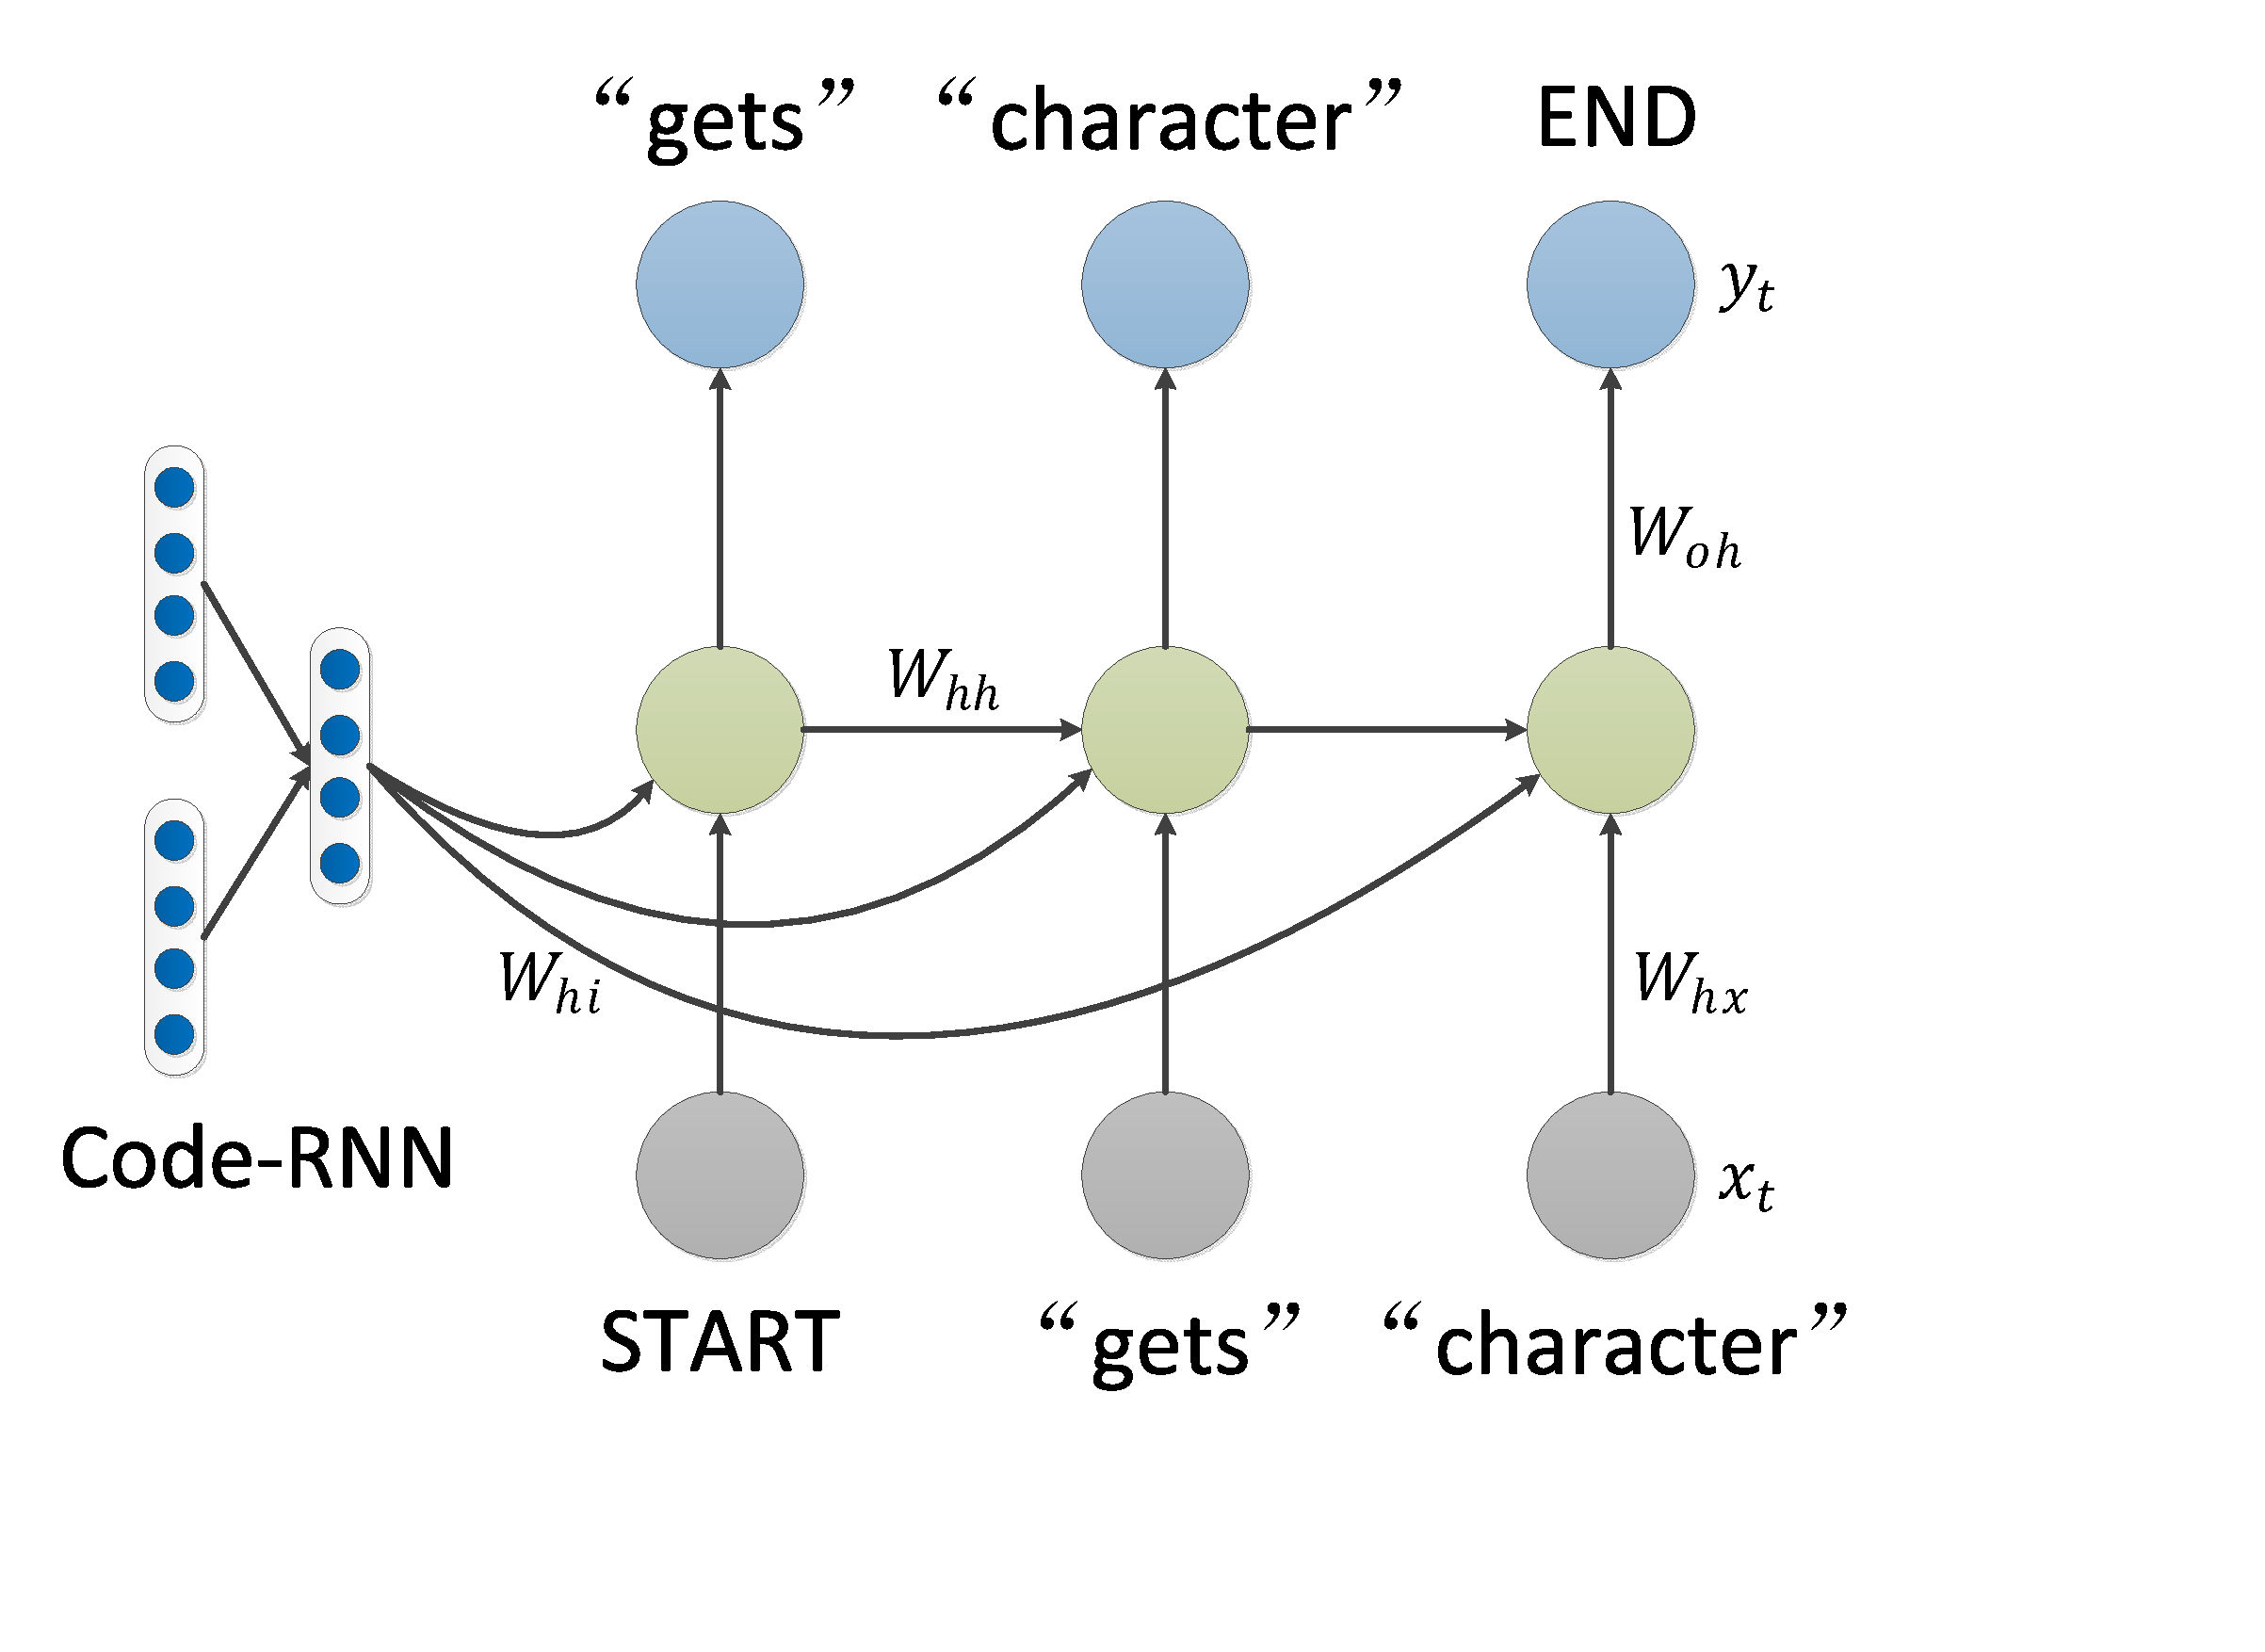
\includegraphics[width=0.8\linewidth]{img/comment_generation.pdf}
\caption{Comment Generation}\label{fig:comment_generate}
\end{figure}

\begin{align}
b_{v} &= W_{hi}[Code\-RNN]\\
h_{t} &= f(W_{hx}x_{t} + W_{hh}h_{t-1} + b_{h} + b_{v})\\
y_{t} &= softmax(W_{oh}h_{t} + b_{o})
\end{align}

When evaluation, we input the ``START'' token at first and choose the maximum probability word as the output. Then from the second step the input words of every step are the output words of previous one step until the output is ``END'' token. So that we can get an automatic generated comment for methods in our model.

